\subsection{\texorpdfstring{\(\tau\)-扩张的类上的群律}{\textbackslash tau-扩张的类上的群律}}

设 \(\mathrm{G}\) 是一个群，\(\mathrm{F}\) 是一个交换群，且 \(\tau : \mathrm{G} \to \mathrm{Aut}(\mathrm{F})\) 是一个群同态。用 \(\delta : \mathrm{G} \to \mathrm{G} \times \mathrm{G}\) 表示对角映射 \(g \mapsto (g, g)\)，并用 \(m : \mathrm{F} \times \mathrm{F} \to \mathrm{F}\) 表示乘法同态 \((f_1, f_2) \mapsto f_1 f_2\)。用 \(s : \mathrm{F} \to \mathrm{F}\) 表示由 \(f \mapsto f^{-1}\) 给出的群同态。设 \(\mathcal{E}_1 = (\Gamma_1, \iota_1, \pi_1)\) 与 \(\mathcal{E}_2 = (\Gamma_2, \iota_2, \pi_2)\) 是 \(\tau\)-扩张（\(\mathrm{G}\) 被 \(\mathrm{F}\) 的）。由于我们有关系

\[
m (((\tau \times \tau) \circ \delta) (g) \cdot (f _ {1}, f _ {2})) = \tau (g) \cdot m (f _ {1}, f _ {2})
\]

（对每个 \(g \in G\) 与所有 \(f_{1}, f_{2} \in F\)），扩张 \(m_{*}(\delta^{*}(\mathcal{E}_{1} \times \mathcal{E}_{2}))\) 是一个 \(\tau\)-扩张；我们称它为 \(\tau\)-扩张 \(E_{1}\) 与 \(E_{2}\) 的积，并记作 \(E_{1}E_{2}\)。这个扩张的类只依赖于扩张 \(E_{1}\) 与 \(E_{2}\) 的类（VIII, 第 288 页，推论 1 与 VIII, 第 291 页，推论 1）。于是这在 \(\operatorname{Ex}_{\tau}(\mathbf{G}, \mathbf{F})\) 上给出一个合成律。

注. —— 设 \(\mathcal{E}_{1}=(\Gamma_{1},\iota_{1},\pi_{1})\) 与 \(\mathcal{E}_{2}=(\Gamma_{2},\iota_{2},\pi_{2})\) 是 G 被 F 的 \(\tau\)-扩张。设 \(\mathcal{E}_{1}\mathcal{E}_{2}=(\Gamma,\iota,\pi)\) 是这些扩张的积。仿照 VIII, 第 289 页的例子，该构造给出一个从纤维积 \(\Gamma_{1}\times_{G}\Gamma_{2}\) 到 \(\Gamma\) 的满射群同态，其核是群同态 \(f\mapsto(\iota_{1}(f),\iota_{2}(f)^{-1})\)（从 F 到 \(\Gamma_{1}\times_{G}\Gamma_{2}\)）的像。

命题 4. —— \(\tau\)-扩张的积赋予集合 \(\mathrm{Ex}_{\tau}(\mathrm{G},\mathrm{F})\) 一个交换群的结构。它的单位元素是半平凡扩张 \(\mathcal{I}_{\tau}\) 的类。\(\tau\)-扩张 \(\mathcal{E}\) 的类的逆元是 \(s_{*}(\mathcal{E})\) 的类。

该律的结合性由诸图的交换性

\pandocbounded{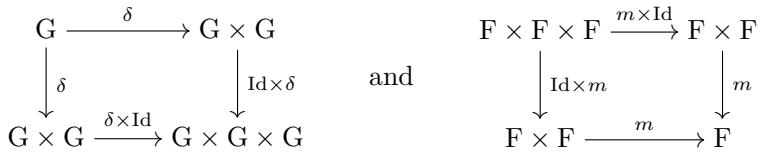
\includegraphics[keepaspectratio]{images/part002_39f17f00.jpg}}

以及 VIII, 第 288 页的推论 2、VIII, 第 291 页的推论 2 与 VIII, 第 292 页的命题 3 得出。

设 \(\Delta : \mathrm{F} \to \mathrm{F} \times \mathrm{F}\) 是对角映射 \(f \mapsto (f, f)\)。设 \(\mathcal{E} = (\Gamma, \iota, \pi)\) 是一个 \(\tau\)-扩张。设 \(\widetilde{\Delta}: \Gamma \to \Gamma \times_{\mathrm{G}} \Gamma\) 是由 \(\gamma \mapsto (\gamma, \gamma)\) 给出的群同态。下图交换：

\pandocbounded{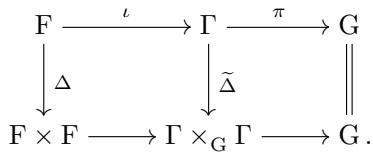
\includegraphics[keepaspectratio]{images/part002_db57599b.jpg}}

由 VIII, 第 290 页的命题 2 推出，\((\tau \times \tau) \circ \delta\)-扩张 \(\delta^{*}(\mathcal{E} \times \mathcal{E})\) 同构于 \(\Delta_{*}(\mathcal{E})\)。

用 \(c: F \to F\) 表示常值同态 \(f \mapsto 1\)。由 VIII, 第 292 页的例 1，\(\mathcal{I}_{\tau}\) 是这个合成律的单位元素这一事实由从 \(\delta^{*}(\mathcal{E} \times \mathcal{E})\) 到 \(\Delta_{*}(\mathcal{E})\) 的同构及交换图

\pandocbounded{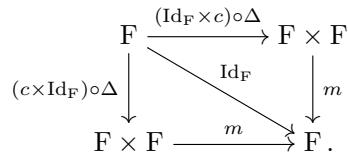
\includegraphics[keepaspectratio]{images/part002_761b87f2.jpg}}

最后一个断言由交换图

\[
\begin{array}{c} \mathrm{F} \xrightarrow {(\mathrm{Id} _ {\mathrm{F}} \times s) \circ \Delta} \mathrm{F} \times \mathrm{F} \\ (s \times \mathrm{Id} _ {\mathrm{F}}) \circ \Delta \Biggl \downarrow \qquad \qquad \qquad \qquad \qquad \qquad \qquad \qquad \qquad \qquad \qquad \qquad \qquad \qquad \qquad \qquad \qquad \qquad \qquad \qquad \qquad \qquad \qquad \qquad \qquad \qquad \qquad \qquad \qquad \qquad \qquad \qquad \qquad \qquad \\ \mathrm{F} \times \mathrm{F} \xrightarrow {m} \mathrm{F}. \end{array}
\]

设 \(\mathcal{E}_1 = (\Gamma_1,\iota_1,\pi_1)\) 与 \(\mathcal{E}_2 = (\Gamma_2,\iota_2,\pi_2)\) 是 \(\tau\)-扩张。群同构 \(\Gamma_1\times \Gamma_2\to \Gamma_2\times \Gamma_1\)（由 \((\gamma_{1},\gamma_{2})\mapsto (\gamma_{2},\gamma_{1})\) 给出）限制为群同构 \(\sigma :\Gamma_1\times_\mathrm{G}\Gamma_2\to \Gamma_2\times_\mathrm{G}\Gamma_1\)。由于关系

\[
\sigma (\iota_ {1} (f), \iota_ {2} (f) ^ {- 1}) = (\iota_ {2} (f ^ {- 1}), \iota_ {1} (f ^ {- 1}) ^ {- 1})
\]

（对 \(f \in F\)），群同态 \(\sigma\) 通过过渡到商诱导出一个 \(\tau\)-扩张的态射（从 \(E_{1}E_{2}\) 到 \(E_{2}E_{1}\) 的）。于是该合成律是交换的。

命题 5. —— a) 设 G 与 G' 是群，并设 F 是一个交换群。设 \(\tau: \mathrm{G} \to \operatorname{Aut}(\mathrm{F})\) 与 \(u: \mathrm{G}' \to \mathrm{G}\) 是群同态。映射 \(u^*: \operatorname{Ex}_{\tau}(\mathrm{G}, \mathrm{F}) \to \operatorname{Ex}_{\tau \circ u}(\mathrm{G}', \mathrm{F})\) 是一个群同态。

\begin{enumerate}
\def\labelenumi{\alph{enumi})}
\setcounter{enumi}{1}
\tightlist
\item
  设 G 是一个群，并设 F 与 \(F'\) 是交换群。设 \(\tau: G \to \text{Aut}(F)\)、\(\tau': G \to \text{Aut}(F')\) 与 \(v: F \to F'\) 是满足
\end{enumerate}

\[
\tau^ {\prime} (g) \cdot v (f) = v (\tau (g) \cdot f)
\]

（对 \(g \in \mathrm{G}\) 与 \(f \in \mathrm{F}\)）的群同态。映射 \(v_{*} : \operatorname{Ex}_{\tau}(\mathrm{G}, \mathrm{F}) \to \operatorname{Ex}_{\tau'}(\mathrm{G}, \mathrm{F}')\) 是一个群同态。

这由诸图的交换性得出

\[
\begin{array}{l} \mathrm{G} ^ {\prime} \xrightarrow {\delta} \mathrm{G} ^ {\prime} \times \mathrm{G} ^ {\prime} \\ \Biggl \downarrow_ {u} \qquad \Biggl \downarrow_ {u \times u} \\ \mathrm{G} \xrightarrow {\delta} \mathrm{G} \times \mathrm{G} \end{array} \qquad \text {and} \qquad \begin{array}{l} \mathrm{F} \times \mathrm{F} \xrightarrow {m} \mathrm{F} \\ \Biggl \downarrow_ {v \times v} \qquad \Biggl \downarrow_ {v} \\ \mathrm{F} ^ {\prime} \times \mathrm{F} ^ {\prime} \xrightarrow {m} \mathrm{F} ^ {\prime}. \end{array}
\]

